% Phase 3 -- written by Huzaifa
% Numbers in the hyperparameter table come from results/hparam_results.csv.
% Training-curve discussion uses results/history_efficientnet.csv.
\section{Phase 3: Model Architecture and Implementation}

\subsection{Framework}
We implemented both models in \textbf{PyTorch} with \textbf{torchvision}.
PyTorch is the usual choice for custom training loops (frozen then unfrozen
stages, early stopping, cosine schedules) and torchvision already ships
EfficientNet-B0 with ImageNet weights. The same scripts run on a Colab T4 GPU
and on CPU. Scikit-learn is left for Phase 4 metrics, not for the networks
themselves.

\subsection{EfficientNet-B0 (transfer learning)}
The main model is torchvision EfficientNet-B0 pretrained on ImageNet
(\texttt{IMAGENET1K\_V1}). The original classifier is replaced by Dropout
then a linear layer to 14 logits. Input tensors are $3 \times 224 \times 224$,
matching the Phase 2 JPEGs. After the backbone, EfficientNet applies global
average pooling to a 1280-dimensional vector, then our head.

Training has two phases, implemented in \texttt{src/train.py}:
\begin{enumerate}
  \item \textbf{Head (5 epochs).} The backbone is frozen. Only Dropout and
        the linear layer are trained, at learning rate $1 \times 10^{-3}$.
  \item \textbf{Fine-tune.} The last 3 entries of \texttt{model.features}
        are unfrozen. Training continues at $1 \times 10^{-4}$ with a fresh
        AdamW optimiser and cosine scheduler, starting from the best head
        checkpoint.
\end{enumerate}
Two stages keep the pretrained filters from being destroyed in the first
epochs, then allow the last blocks to adapt to desi food photos.

\begin{figure}[H]
  \centering
  \begin{tikzpicture}[
      font=\small,
      box/.style={draw, rounded corners, align=center, minimum height=1.05cm, inner sep=4pt},
      arr/.style={-{Latex}, thick}
    ]
    \node[box, minimum width=2.4cm] (in) {Input\\$3 \times 224 \times 224$};
    \node[box, minimum width=3.6cm, right=0.45cm of in] (bb) {EfficientNet-B0\\backbone\\{\scriptsize frozen, then last 3 blocks}};
    \node[box, minimum width=2.2cm, right=0.45cm of bb] (gap) {Global avg.\\pool (1280)};
    \node[box, minimum width=1.8cm, right=0.45cm of gap] (drop) {Dropout};
    \node[box, minimum width=2.0cm, right=0.45cm of drop] (fc) {Linear\\14 logits};
    \draw[arr] (in) -- (bb);
    \draw[arr] (bb) -- (gap);
    \draw[arr] (gap) -- (drop);
    \draw[arr] (drop) -- (fc);
  \end{tikzpicture}
  \caption{EfficientNet-B0 transfer pipeline used in \texttt{src/efficientnet\_model.py}.}
\end{figure}

\subsection{Baseline CNN}
\texttt{src/baseline\_cnn.py} is Abdullah's from-scratch network. The shared
contract is the same I/O as EfficientNet: class \texttt{BaselineCNN(num\_classes=14)},
input $3 \times 224 \times 224$, output 14 logits, trained with
\texttt{python src/train.py --model baseline}.

The layer table, block diagram and hyperparameters of the baseline are in
Phase~4, so they are not repeated here.

\subsection{Loss, optimiser, schedule, regularisation}
\begin{itemize}
  \item \textbf{Loss.} Cross-entropy with label smoothing $0.1$. Smoothing
        stops the head from becoming over-confident on noisy Bing labels
        (Phase 2 noted watermarks and a little label noise).
  \item \textbf{Optimiser.} AdamW on \emph{trainable} parameters only, with
        weight decay $1 \times 10^{-4}$. AdamW is the usual default for
        transformer and CNN fine-tuning; excluding frozen weights avoids
        useless states in the optimiser.
  \item \textbf{Scheduler.} Cosine annealing over the epochs of each phase.
        The learning rate falls smoothly and does not need an extra validation
        rule (unlike ReduceLROnPlateau).
  \item \textbf{Early stopping.} Training watches validation loss with
        patience 5 and writes the best weights under \texttt{checkpoints/}
        as \texttt{efficientnet\_best.pt}.
  \item \textbf{Augmentation (train only).} RandomResizedCrop 224 (scale
        $0.8$--$1.0$), horizontal flip, rotation of about $15^{\circ}$, and
        ColorJitter (brightness and contrast $0.2$). Validation and test
        only resize to $224 \times 224$.
  \item \textbf{Normalisation.} ImageNet mean $(0.485, 0.456, 0.406)$ and
        std $(0.229, 0.224, 0.225)$, as named constants in
        \texttt{src/dataset.py}. Phase 2 saved train-set statistics in
        \texttt{norm\_stats.json} and said they ``will be used''. We do
        \emph{not} use those stats, because the EfficientNet weights were
        pretrained with ImageNet normalisation; mixing the two scales would
        shift every activation in the frozen backbone.
\end{itemize}

\subsection{Hyperparameter search}
\texttt{src/tune.py} changes \emph{one} factor at a time around a default
(head lr $1 \times 10^{-3}$, fine-tune lr $1 \times 10^{-4}$, batch 32,
dropout $0.3$, weight decay $1 \times 10^{-4}$, label smoothing $0.1$).
Each trial ran at most 8 epochs on a Colab T4, without writing a test-pred
file. Table~\ref{tab:hparam} is copied from \texttt{results/hparam\_results.csv}.
The best row (lowest validation loss) is in bold.

\begin{table}[H]
  \centering
  \small
  \begin{tabular}{|l|r|r|r|r|r|}
    \hline
    \textbf{Run} & \textbf{lr} & \textbf{Batch} & \textbf{Drop.} & \textbf{Val.\ loss} & \textbf{Val.\ acc.} \\
    \hline
    default      & 0.001  & 32 & 0.3 & 1.190 & 0.777 \\
    lr\_3e-4     & 0.0003 & 32 & 0.3 & 1.194 & 0.773 \\
    lr\_1e-4     & 0.0001 & 32 & 0.3 & 1.238 & 0.767 \\
    \textbf{batch\_16} & \textbf{0.001} & \textbf{16} & \textbf{0.3} & \textbf{1.167} & \textbf{0.792} \\
    batch\_64    & 0.001  & 64 & 0.3 & 1.217 & 0.769 \\
    dropout\_0.2 & 0.001  & 32 & 0.2 & 1.187 & 0.781 \\
    dropout\_0.5 & 0.001  & 32 & 0.5 & 1.200 & 0.775 \\
    wd\_1e-2     & 0.001  & 32 & 0.3 & 1.190 & 0.777 \\
    \hline
  \end{tabular}
  \caption{One-factor EfficientNet search (\texttt{results/hparam\_results.csv}).
  Fine-tune lr $1 \times 10^{-4}$, weight decay $1 \times 10^{-4}$ except
  \texttt{wd\_1e-2} ($1 \times 10^{-2}$), label smoothing $0.1$ throughout.
  Accuracies are the CSV \texttt{best\_val\_acc} values.}
  \label{tab:hparam}
\end{table}

Lowering the head learning rate or raising the batch size made validation
loss worse than the default. Dropout $0.2$ was slightly better than $0.3$ on
accuracy but not on loss. Weight decay $1 \times 10^{-2}$ matched the default
loss. \textbf{Batch size 16} was the only change that clearly reduced
validation loss (1.167 vs 1.190), so the final EfficientNet run used that
batch size and otherwise the default knobs: 20 epochs, 5 head epochs, last 3
blocks unfrozen, dropout $0.3$, AdamW weight decay $1 \times 10^{-4}$, label
smoothing $0.1$.

From \texttt{results/history\_efficientnet.csv}, that full run reached its
best validation loss at epoch 19 (loss 1.069, accuracy 0.830) during
fine-tuning. Test-set Precision, Recall, F1 and AUC are Phase 4
(\texttt{evaluate.py}); they are not computed in \texttt{train.py}.

\subsection{Training curves}
Figure~\ref{fig:curves-eff} is \texttt{results/curves\_efficientnet.png}.
Loss and accuracy are plotted for train and validation. The dashed line marks
the first fine-tune epoch (epoch 6). Both curves improve after that line,
which is the point of unfreezing the last blocks.

\begin{figure}[H]
  \centering
  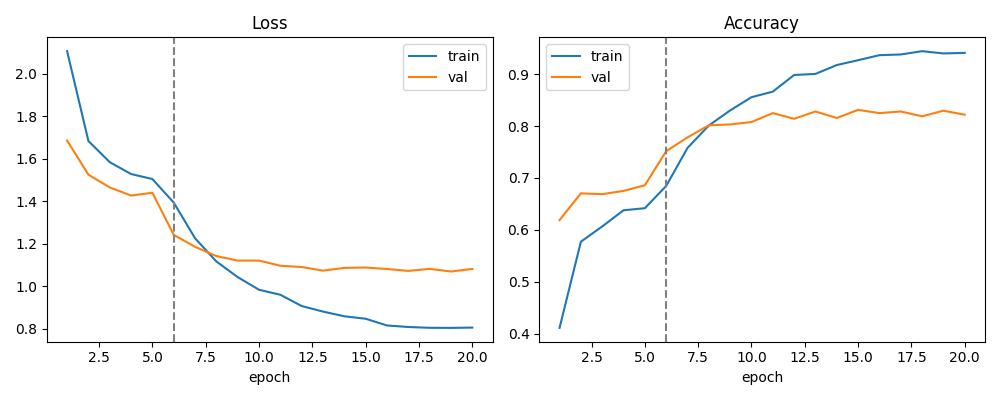
\includegraphics[width=0.95\textwidth]{curves_efficientnet.png}
  \caption{EfficientNet-B0 train/val loss and accuracy
  (\texttt{results/curves\_efficientnet.png}, final 20-epoch run, batch 16).}
  \label{fig:curves-eff}
\end{figure}

The baseline's curves are in Phase~4 (\texttt{results/curves\_baseline.png}).
